\documentclass[aspectratio=169,11pt]{beamer}

\usetheme{Madrid}
\usecolortheme{default}

\usepackage[T1]{fontenc}
\usepackage[utf8]{inputenc}
\usepackage{amsmath,amssymb,booktabs,tabularx}
\usepackage{tikz}
\usepackage{pgfplots}
\usepackage{url}
\usetikzlibrary{arrows.meta,positioning,calc,fit,shapes.geometric}
\pgfplotsset{compat=1.18}

\definecolor{CrossNavy}{HTML}{102A43}
\definecolor{CrossBlue}{HTML}{147D92}
\definecolor{CrossTeal}{HTML}{2A9D8F}
\definecolor{CrossGold}{HTML}{E9A23B}
\definecolor{CrossRed}{HTML}{C8553D}
\definecolor{CrossPale}{HTML}{EAF2F5}
\definecolor{CrossGray}{HTML}{627D98}

\setbeamercolor{structure}{fg=CrossBlue}
\setbeamercolor{frametitle}{fg=white,bg=CrossNavy}
\setbeamercolor{title}{fg=CrossNavy}
\setbeamercolor{block title}{fg=white,bg=CrossBlue}
\setbeamercolor{block body}{fg=CrossNavy,bg=CrossPale}
\setbeamercolor{alerted text}{fg=CrossRed}
\setbeamertemplate{navigation symbols}{}
\setbeamertemplate{footline}[frame number]
\setbeamersize{text margin left=8mm,text margin right=8mm}

\title[CrossLayer Progress]{Network-Aware Workload Placement in Kubernetes}
\subtitle{CrossLayer: measured telemetry, explainable affinity, and the next research steps}
\author{Presenter: \textbf{[Your Name]}}
\institute{[Department / University]}
\date{Presentation \textbullet\ 13 November 2026}

\newcommand{\statusdone}{\textcolor{CrossTeal}{\textbf{DONE}}}
\newcommand{\statusactive}{\textcolor{CrossGold}{\textbf{IN PROGRESS}}}
\newcommand{\statusfuture}{\textcolor{CrossGray}{\textbf{PLANNED}}}
\newcommand{\smallsource}[1]{\par\vspace{1mm}{\tiny\textcolor{CrossGray}{#1}}}
\newcommand{\say}[1]{\note{\small #1}}

\begin{document}

\begin{frame}
  \titlepage
  \say{Introduce the project as a research prototype, not an automatic production scheduler. The emphasis so far has been to build trustworthy measurements first, then use them in an explainable network-affinity baseline.}
\end{frame}

\begin{frame}{The research problem}
  \begin{columns}[T,onlytextwidth]
    \column{0.56\textwidth}
      \begin{block}{Why placement matters}
        A microservice request may cross several network hops. Placing communicating
        services on better-connected nodes may reduce network cost, but placement
        decisions must be based on observed traffic and measured network conditions.
      \end{block}
      \vspace{2mm}
      \textbf{Research question}\\
      Can live cluster and service telemetry support an explainable ranking of
      Kubernetes nodes for a communicating workload?
    \column{0.40\textwidth}
      \begin{alertblock}{Scope for this milestone}
        \begin{itemize}
          \item Measure cluster and network state.
          \item Connect observed service calls to node-to-node quality.
          \item Rank candidate nodes transparently.
          \item Keep all recommendations advisory.
        \end{itemize}
      \end{alertblock}
  \end{columns}
  \say{The order is deliberate: data collection and a reproducible mathematical baseline come before machine learning or automated migration.}
\end{frame}

\begin{frame}{System architecture: from cluster measurements to dashboard}
  \centering
  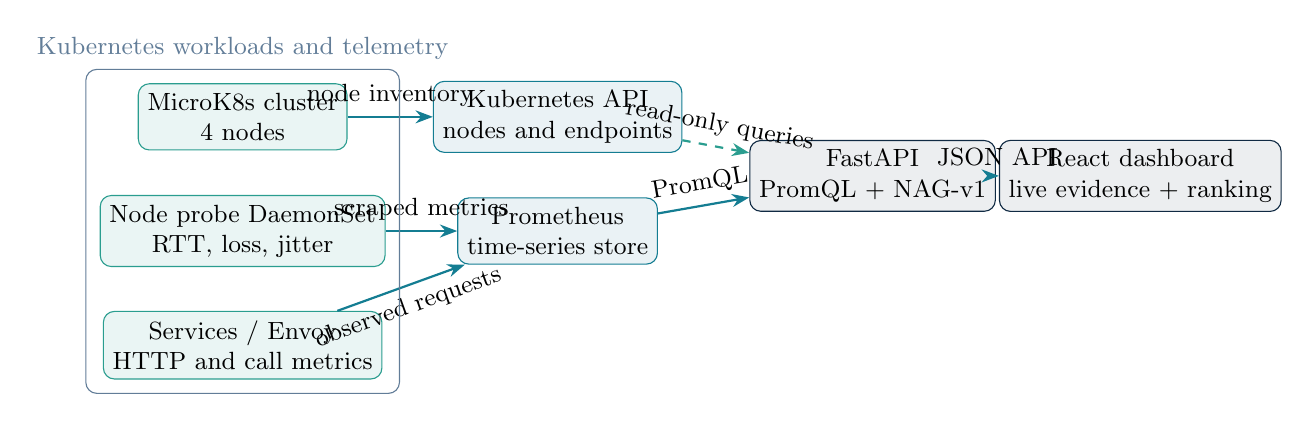
\begin{tikzpicture}[
    font=\small,
    block/.style={draw=CrossBlue,fill=CrossPale,rounded corners,align=center,
      minimum width=2.45cm,minimum height=0.82cm},
    source/.style={draw=CrossTeal,fill=CrossTeal!10,rounded corners,align=center,
      minimum width=2.55cm,minimum height=0.82cm},
    result/.style={draw=CrossNavy,fill=CrossNavy!8,rounded corners,align=center,
      minimum width=2.5cm,minimum height=0.82cm},
    arr/.style={-{Stealth[length=2.2mm]},thick,draw=CrossBlue},
    readarr/.style={-{Stealth[length=2.2mm]},thick,dashed,draw=CrossTeal}
  ]
    \node[source] (cluster) at (0,2.1) {MicroK8s cluster\\4 nodes};
    \node[source] (probe) at (0,0.65) {Node probe DaemonSet\\RTT, loss, jitter};
    \node[source] (apps) at (0,-0.8) {Services / Envoy\\HTTP and call metrics};
    \node[block] (prom) at (4.0,0.65) {Prometheus\\time-series store};
    \node[block] (kube) at (4.0,2.1) {Kubernetes API\\nodes and endpoints};
    \node[result] (api) at (8.0,1.35) {FastAPI\\PromQL + NAG-v1};
    \node[result] (ui) at (11.4,1.35) {React dashboard\\live evidence + ranking};

    \draw[arr] (cluster) -- node[above,sloped]{node inventory} (kube);
    \draw[arr] (probe) -- node[above]{scraped metrics} (prom);
    \draw[arr] (apps) -- node[below,sloped]{observed requests} (prom);
    \draw[readarr] (kube) -- node[above,sloped]{read-only queries} (api);
    \draw[arr] (prom) -- node[above,sloped]{PromQL} (api);
    \draw[arr] (api) -- node[above]{JSON API} (ui);

    \node[draw=CrossGray,rounded corners,inner sep=5pt,fit=(cluster)(probe)(apps),
      label={[CrossGray]above:Kubernetes workloads and telemetry}] {};
  \end{tikzpicture}
  \vspace{3mm}
  \begin{center}
    \small The dashboard reads measurements; NAG-v1 does \textbf{not} issue Kubernetes placement changes.
  \end{center}
  \say{Walk left to right: the Kubernetes API supplies topology and endpoints; Prometheus supplies time series; the backend joins the evidence; the UI labels measured versus derived results.}
\end{frame}

\begin{frame}{Progress so far}
  \begin{columns}[T,onlytextwidth]
    \column{0.49\textwidth}
      \begin{block}{Implemented and verified}
        \begin{itemize}
          \item FastAPI backend and React dashboard with typed measured / derived / unavailable states.
          \item Read-only access to Kubernetes and Prometheus through local tunnels.
          \item Node, Pod, compute, network, Envoy, dependency, and experiment views.
          \item Inter-node ICMP probe exporter and Prometheus metrics.
          \item NAG-v1 score, traffic-aware ranking, explanation, and tests.
        \end{itemize}
      \end{block}
    \column{0.47\textwidth}
      \begin{alertblock}{Important qualification}
        \begin{itemize}
          \item Experiment services are isolated from existing workloads.
          \item The load control is capped and requires an explicit start.
          \item Only a small number of smoke requests have been sent.
          \item A sustained load evaluation has \textbf{not} been run.
          \item No measured service dependency edges were present in the latest live affinity check.
        \end{itemize}
      \end{alertblock}
  \end{columns}
  \say{Say clearly that implementation progress and evaluation progress are different. The pipeline and baseline are working; controlled, repeated workload experiments are the next major evidence-gathering step.}
\end{frame}

\begin{frame}{Live cluster snapshot}
  \begin{columns}[T,onlytextwidth]
    \column{0.37\textwidth}
      \begin{block}{Verified live API response}
        \centering
        {\Huge\textcolor{CrossBlue}{4}}\\[-1mm]
        \small Kubernetes nodes\\[2mm]
        {\Huge\textcolor{CrossTeal}{4/4}}\\[-1mm]
        \small active probe targets\\[2mm]
        {\Huge\textcolor{CrossBlue}{12}}\\[-1mm]
        \small directed node links\\[2mm]
        {\Huge\textcolor{CrossGold}{0}}\\[-1mm]
        \small measured service edges / recommendations
      \end{block}
      \smallsource{Snapshot checked against the live API on 12 Nov 2026. Values can change as the cluster changes.}
    \column{0.60\textwidth}
      \centering
      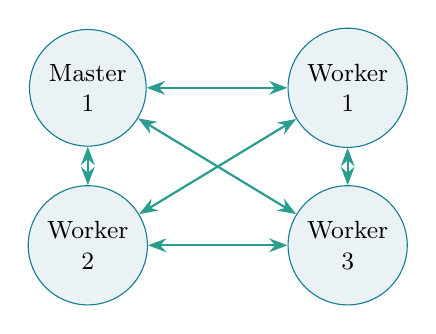
\begin{tikzpicture}[
        font=\small,
        node/.style={circle,draw=CrossBlue,fill=CrossPale,minimum size=1.35cm,align=center},
        conn/.style={<->,>=Stealth,draw=CrossTeal,thick}
      ]
        \node[node] (n1) at (0,2.0) {Master\\1};
        \node[node] (n2) at (3.3,2.0) {Worker\\1};
        \node[node] (n3) at (0,0) {Worker\\2};
        \node[node] (n4) at (3.3,0) {Worker\\3};
        \draw[conn] (n1) -- (n2);
        \draw[conn] (n1) -- (n3);
        \draw[conn] (n1) -- (n4);
        \draw[conn] (n2) -- (n3);
        \draw[conn] (n2) -- (n4);
        \draw[conn] (n3) -- (n4);
      \end{tikzpicture}
      \vspace{1mm}
      \begin{center}
        \small Six node pairs, measured in both directions\\
        \textcolor{CrossGray}{The drawing shows coverage, not relative link quality.}
      \end{center}
  \end{columns}
  \say{The four probes are up and all 12 directed node-to-node links have measured features. Service traffic is a separate input: without observed request edges there is no evidence-based workload placement recommendation.}
\end{frame}

\begin{frame}{Measurement pipeline and controlled services}
  \centering
  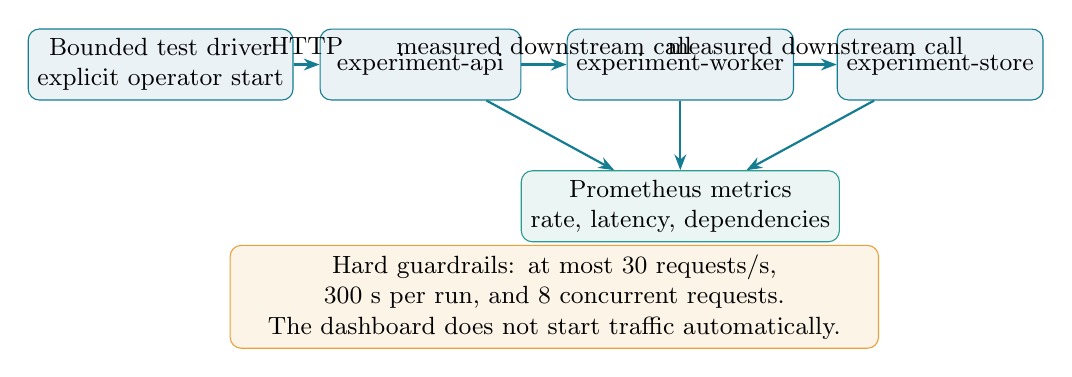
\begin{tikzpicture}[
    font=\small,
    svc/.style={draw=CrossBlue,fill=CrossPale,rounded corners,minimum width=2.55cm,
      minimum height=0.9cm,align=center},
    metric/.style={draw=CrossTeal,fill=CrossTeal!10,rounded corners,minimum width=2.6cm,
      minimum height=0.9cm,align=center},
    arr/.style={-{Stealth[length=2mm]},thick,draw=CrossBlue}
  ]
    \node[svc] (load) at (0,1.4) {Bounded test driver\\explicit operator start};
    \node[svc] (api) at (3.3,1.4) {experiment-api};
    \node[svc] (worker) at (6.6,1.4) {experiment-worker};
    \node[svc] (store) at (9.9,1.4) {experiment-store};
    \node[metric] (prom) at (6.6,-0.4) {Prometheus metrics\\rate, latency, dependencies};
    \draw[arr] (load) -- node[above]{HTTP} (api);
    \draw[arr] (api) -- node[above]{measured downstream call} (worker);
    \draw[arr] (worker) -- node[above]{measured downstream call} (store);
    \draw[arr] (api) -- (prom);
    \draw[arr] (worker) -- (prom);
    \draw[arr] (store) -- (prom);
    \node[draw=CrossGold,rounded corners,fill=CrossGold!12,align=center,
      text width=8cm] at (5.0,-1.55)
      {Hard guardrails: at most 30 requests/s, 300 s per run, and 8 concurrent requests.\\
       The dashboard does not start traffic automatically.};
  \end{tikzpicture}
  \vspace{3mm}
  \begin{itemize}
    \item The services are isolated in the experiment namespace and expose request and dependency metrics.
    \item The probe DaemonSet separately measures low-rate node-to-node ICMP telemetry.
    \item \textbf{Current evidence gap:} no sustained load campaign has yet populated the dependency graph.
  \end{itemize}
  \say{Explain the distinction between synthetic test traffic and synthetic telemetry: a controlled workload is an explicit experiment, but the reported measurements still come from Prometheus observations.}
\end{frame}

\begin{frame}{NAG-v1: explainable measured link affinity}
  \small
  Let $M_{ij}$ be the set of features actually observed from node $i$ to node $j$.
  Each available feature is normalized to $[0,1]$:
  \[
    \begin{aligned}
      q_{\text{lat}} &= e^{-\mathrm{RTT}_{p95}/10\mathrm{ms}}, &
      q_{\text{loss}} &= 1-\mathrm{loss}/100,\\
      q_{\text{jitter}} &= e^{-\mathrm{jitter}/5\mathrm{ms}}, &
      q_{\text{cong}} &= 1-\frac{\max(u_i,u_j)}{100}.
    \end{aligned}
  \]
  \[
    A_{ij}=100\,
    \frac{\sum_{k\in M_{ij}} w_k q_k}
         {\sum_{k\in M_{ij}} w_k},
    \qquad
    C_{ij}=100\,
    \frac{\sum_{k\in M_{ij}} w_k}{\sum_k w_k}.
  \]
  \begin{columns}[T,onlytextwidth]
    \column{0.56\textwidth}
      \begin{block}{Interpretation}
        $A_{ij}$ is a 0--100 quality score for the \textbf{directed} link.
        $C_{ij}$ is the percentage of configured network-feature weight supported by measurements.
      \end{block}
    \column{0.40\textwidth}
      \begin{alertblock}{Missing data policy}
        Missing metrics are omitted and weights renormalized. They are never fabricated or silently set to zero.
      \end{alertblock}
  \end{columns}
  \say{Emphasize that the score is derived, not a directly measured physical quantity. It is interpretable because each contribution and the measurement coverage are visible.}
\end{frame}

\begin{frame}{Features and current model coverage}
  \begin{columns}[T,onlytextwidth]
    \column{0.56\textwidth}
      \centering
      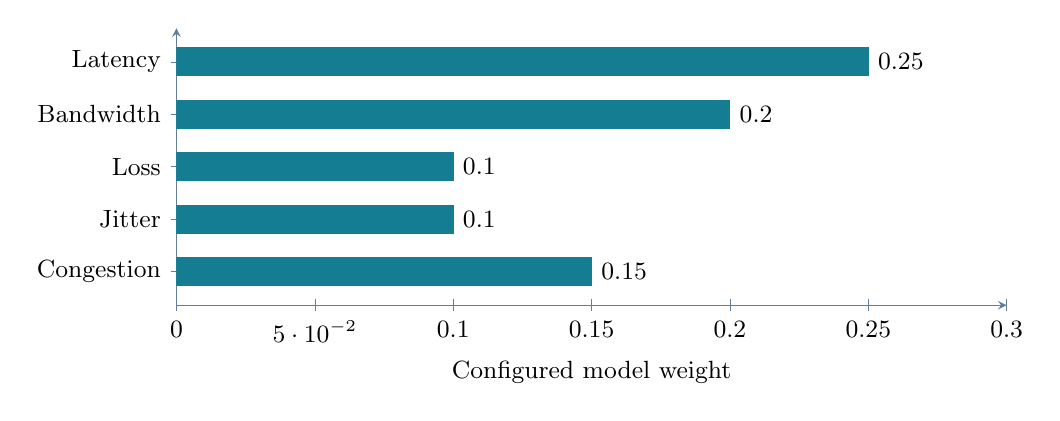
\begin{tikzpicture}
        \begin{axis}[
          xbar,
          width=\linewidth,
          height=5.1cm,
          xmin=0,xmax=0.30,
          xlabel={Configured model weight},
          symbolic y coords={Congestion,Jitter,Loss,Bandwidth,Latency},
          ytick=data,
          nodes near coords,
          nodes near coords align={horizontal},
          every node near coord/.append style={font=\small},
          bar width=10pt,
          axis x line=bottom,
          axis y line=left,
          tick label style={font=\small},
          label style={font=\small},
          xtick={0,0.05,0.10,0.15,0.20,0.25,0.30},
          enlarge y limits=0.16,
          axis line style={CrossGray},
          tick style={CrossGray}
        ]
          \addplot[fill=CrossBlue,draw=CrossBlue] coordinates {
            (0.25,Latency) (0.20,Bandwidth) (0.10,Loss)
            (0.10,Jitter) (0.15,Congestion)
          };
        \end{axis}
      \end{tikzpicture}
    \column{0.41\textwidth}
      \begin{block}{What is available now}
        RTT p95, packet loss, jitter, and physical-interface utilization are queried from active probes and node metrics.
      \end{block}
      \begin{alertblock}{Bandwidth is not measured}
        A configured bandwidth weight of 0.20 is reserved, but available capacity is not collected yet. The observed weights total 0.60 of 0.80 network weight, giving 75\% feature coverage when all four current signals are present.
      \end{alertblock}
      \smallsource{Bars are configured weights, not measured link values.}
  \end{columns}
  \say{The bar chart shows design weights rather than live performance. Clarify that bandwidth is a missing feature, not a zero-throughput link.}
\end{frame}

\begin{frame}{From service calls to candidate-node ranking}
  \begin{columns}[T,onlytextwidth]
    \column{0.49\textwidth}
      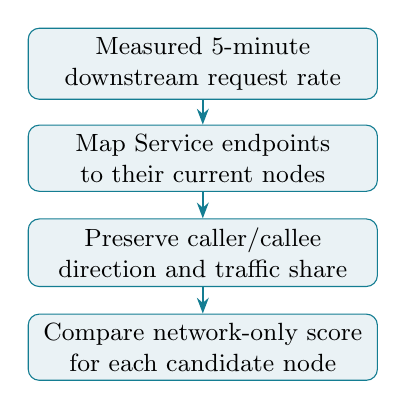
\begin{tikzpicture}[
        font=\small,
        box/.style={draw=CrossBlue,fill=CrossPale,rounded corners,align=center,
          text width=4.2cm,minimum height=0.8cm},
        arr/.style={-{Stealth[length=2mm]},thick,draw=CrossBlue}
      ]
        \node[box] (a) at (0,3.0) {Measured 5-minute downstream request rate};
        \node[box] (b) at (0,1.8) {Map Service endpoints to their current nodes};
        \node[box] (c) at (0,0.6) {Preserve caller/callee direction and traffic share};
        \node[box] (d) at (0,-0.6) {Compare network-only score for each candidate node};
        \draw[arr] (a) -- (b);
        \draw[arr] (b) -- (c);
        \draw[arr] (c) -- (d);
      \end{tikzpicture}
    \column{0.47\textwidth}
      \begin{block}{Traffic-weighted placement score}
        For candidate node $x$ and observed peer paths $e$:
        \[
          P(x)=\frac{\sum_e r_e A_e(x)}{\sum_e r_e},
        \]
        where $r_e$ is the measured request rate and $A_e(x)$ is the directed link affinity if that path is covered.
      \end{block}
      \begin{alertblock}{Advisory gates}
        $\geq 80\%$ traffic coverage, $\geq 50\%$ measured-feature coverage, and $\geq 5$ score points of improvement over current placement.
      \end{alertblock}
      \small These thresholds are initial research choices, not calibrated policy.
  \end{columns}
  \say{For outgoing replicas, observed per-Pod rates distribute traffic; if unavailable, equal sharing is an explicitly labeled approximation. Same-node peers are treated as a topology assumption and contribute zero measured-feature coverage.}
\end{frame}

\begin{frame}{What the dashboard currently shows}
  \begin{columns}[T,onlytextwidth]
    \column{0.58\textwidth}
      \centering
      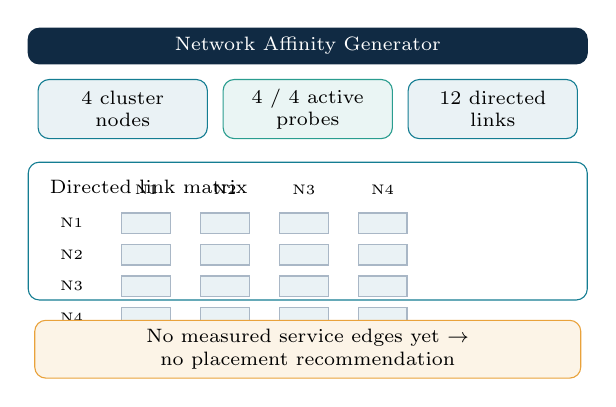
\begin{tikzpicture}[font=\scriptsize]
        \node[draw=CrossNavy,fill=CrossNavy,text=white,rounded corners,
          minimum width=7.1cm,minimum height=0.42cm] at (3.55,3.7)
          {Network Affinity Generator};
        \node[draw=CrossBlue,fill=CrossPale,rounded corners,align=center,
          minimum width=2.15cm,minimum height=0.75cm] at (1.2,2.9)
          {4 cluster\\nodes};
        \node[draw=CrossTeal,fill=CrossTeal!10,rounded corners,align=center,
          minimum width=2.15cm,minimum height=0.75cm] at (3.55,2.9)
          {4 / 4 active\\probes};
        \node[draw=CrossBlue,fill=CrossPale,rounded corners,align=center,
          minimum width=2.15cm,minimum height=0.75cm] at (5.9,2.9)
          {12 directed\\links};
        \node[draw=CrossBlue,rounded corners,minimum width=7.1cm,
          minimum height=1.75cm] (matrix) at (3.55,1.35) {};
        \node[anchor=north west] at (0.15,2.12) {Directed link matrix};
        \foreach \x/\lab in {1.5/N1,2.5/N2,3.5/N3,4.5/N4} {
          \node[font=\tiny] at (\x,1.88) {\lab};
        }
        \foreach \y/\lab in {1.45/N1,1.05/N2,0.65/N3,0.25/N4} {
          \node[font=\tiny] at (0.55,\y) {\lab};
        }
        \foreach \x in {1.5,2.5,3.5,4.5} {
          \foreach \y in {1.45,1.05,0.65,0.25} {
            \fill[CrossPale] (\x-0.31,\y-0.13) rectangle (\x+0.31,\y+0.13);
            \draw[CrossGray!55] (\x-0.31,\y-0.13) rectangle (\x+0.31,\y+0.13);
          }
        }
        \node[draw=CrossGold,fill=CrossGold!12,rounded corners,
          text width=6.7cm,align=center] at (3.55,-0.15)
          {No measured service edges yet $\rightarrow$ no placement recommendation};
      \end{tikzpicture}
      \smallsource{Schematic of the live dashboard panels. Matrix cells intentionally contain no invented scores.}
    \column{0.38\textwidth}
      \begin{itemize}
        \item Active probe targets and node inventory.
        \item Directed node-affinity matrix and feature coverage.
        \item Measured service edges, when calls are observed.
        \item Candidate ranking, evidence, and threshold explanation.
        \item Unavailable states rather than placeholder results.
      \end{itemize}
      \vspace{2mm}
      \textbf{Live UI:} \url{http://127.0.0.1:5174/affinity}
  \end{columns}
  \say{The schematic is deliberately not a screenshot or a source of numeric scores. It communicates what the UI displays and why the dependency area is currently empty.}
\end{frame}

\begin{frame}{Verification and reproducibility}
  \begin{columns}[T,onlytextwidth]
    \column{0.47\textwidth}
      \begin{block}{Software verification}
        \begin{itemize}
          \item 29 backend tests passed.
          \item Frontend TypeScript check and production build passed.
          \item Live API returned 4 nodes, 12 links, and 4/4 active probes.
          \item Prometheus and Kubernetes health checks both succeeded.
        \end{itemize}
      \end{block}
    \column{0.49\textwidth}
      \begin{alertblock}{What these checks do not prove}
        \begin{itemize}
          \item They are not a sustained performance evaluation.
          \item They do not calibrate score weights or thresholds.
          \item They do not show that NAG-v1 improves application SLOs.
          \item They do not validate a real workload migration.
        \end{itemize}
      \end{alertblock}
  \end{columns}
  \vspace{2mm}
  \small Test evidence verifies implementation behavior and live connectivity; scientific evaluation remains future work.
  \say{Be precise: passing tests establish correctness of tested behavior, not superiority of the proposed algorithm.}
\end{frame}

\begin{frame}{Planned evaluation: controlled, repeatable, and safe}
  \begin{enumerate}
    \item Record a quiet-cluster baseline and verify all collectors and experiment services are healthy.
    \item Run a short, low-rate smoke step; proceed only if cluster health remains normal.
    \item Increase offered request rate in controlled steps; repeat each setting at least three times.
    \item Record offered/completed requests, errors, p50/p95/p99 latency, downstream calls, node placement, RTT, loss, jitter, CPU, and memory.
    \item Compare current placement with network-only NAG-v1 recommendations offline; do not migrate workloads during initial evaluation.
  \end{enumerate}
  \begin{block}{Safety envelope already enforced by the experiment controller}
    Maximum 30 requests/s \quad | \quad Maximum 300 seconds/run \quad | \quad Maximum 8 concurrent requests
  \end{block}
  \smallsource{Exact experiment rates and durations should be selected with the supervisor and adjusted to cluster health; no sustained run has been completed yet.}
  \say{Explain that the experimental controller has hard caps, but a cap is not a target. Begin conservatively and stop on elevated errors or unhealthy services.}
\end{frame}

\begin{frame}{Roadmap: from baseline to validated research}
  \centering
  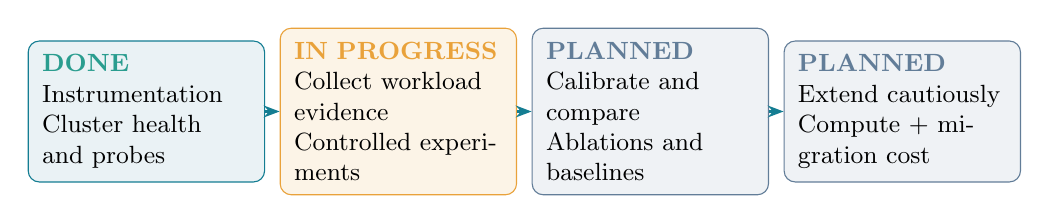
\begin{tikzpicture}[
    font=\small,
    phase/.style={draw=CrossBlue,fill=CrossPale,rounded corners,
      text width=2.65cm,minimum height=1.65cm,align=left,inner sep=5pt},
    active/.style={draw=CrossGold,fill=CrossGold!12,rounded corners,
      text width=2.65cm,minimum height=1.65cm,align=left,inner sep=5pt},
    future/.style={draw=CrossGray,fill=CrossGray!10,rounded corners,
      text width=2.65cm,minimum height=1.65cm,align=left,inner sep=5pt},
    arr/.style={-{Stealth[length=2mm]},thick,draw=CrossBlue}
  ]
    \node[phase] (p1) at (1.8,1.6) {\statusdone\\Instrumentation\\Cluster health and probes};
    \node[active] (p2) at (5.0,1.6) {\statusactive\\Collect workload evidence\\Controlled experiments};
    \node[future] (p3) at (8.2,1.6) {\statusfuture\\Calibrate and compare\\Ablations and baselines};
    \node[future] (p4) at (11.4,1.6) {\statusfuture\\Extend cautiously\\Compute + migration cost};
    \draw[arr] (p1) -- (p2);
    \draw[arr] (p2) -- (p3);
    \draw[arr] (p3) -- (p4);
  \end{tikzpicture}
  \vspace{5mm}
  \begin{columns}[T,onlytextwidth]
    \column{0.49\textwidth}
      \begin{block}{Near-term research}
        Populate measured dependency edges; add bandwidth measurement; validate directionality, replica traffic distribution, and score coverage.
      \end{block}
    \column{0.49\textwidth}
      \begin{block}{Later comparisons}
        Compare current placement, latency-only ranking, weighted NAG-v1, and (only with enough data) graph or multi-criteria alternatives.
      \end{block}
  \end{columns}
  \say{Graph methods, TOPSIS, adaptive weights, and prediction are candidate comparisons, not promised improvements. First build enough labeled, repeated data to test them fairly.}
\end{frame}

\begin{frame}{Limitations and safety boundaries}
  \begin{itemize}
    \item The current affinity score is \textbf{network-only}; it does not yet include CPU/memory fit, taints, volumes, security/data locality, migration cost, or application SLOs.
    \item Bandwidth capacity is not currently scored; equal replica-share fallback is an approximation when per-Pod rates are absent.
    \item Same-node paths are topology assumptions, not measured inter-node links.
    \item Current metric labels do not provide cross-namespace caller attribution.
    \item Weights, normalization scales, and coverage thresholds are starting hypotheses that need calibration and sensitivity analysis.
    \item NAG-v1 is advisory only. Automated scheduling or migration is out of scope until extensive offline validation, dry-run checks, and explicit approval.
  \end{itemize}
  \begin{alertblock}{Core principle}
    If telemetry is missing, show the limitation. Do not invent measurements, scores, or recommendations.
  \end{alertblock}
  \say{These limitations define the research work rather than weaken the result. They identify what must be measured and controlled before making broader claims.}
\end{frame}

\begin{frame}{Summary and discussion}
  \begin{enumerate}
    \item A live telemetry-to-dashboard pipeline is connected to a four-node MicroK8s cluster.
    \item Inter-node probes are active and NAG-v1 produces explainable directed link scores.
    \item The missing piece is measured workload communication under controlled, repeated experiments.
    \item Next: collect that evidence, evaluate against baselines, calibrate the model, and keep placement advice offline and safe.
  \end{enumerate}
  \vfill
  \begin{center}
    {\Large\textcolor{CrossBlue}{Thank you}}\\[2mm]
    {\large Questions and feedback}
  \end{center}
  \say{Invite feedback on the proposed evaluation design and which baseline comparisons the professor expects.}
\end{frame}

\begin{frame}{Presenter quick-reference}
  \small
  \begin{tabularx}{\textwidth}{>{\bfseries}p{0.23\textwidth}X}
    If asked: ``Is the affinity score measured?'' &
      No. It is a derived score whose inputs are measured; coverage and assumptions are shown.\\[2mm]
    If asked: ``Why no recommendation?'' &
      No measured service-dependency edges were present in the live snapshot, so traffic-weighted placement ranking is not justified yet.\\[2mm]
    If asked: ``Is this ML?'' &
      No. NAG-v1 is an explainable mathematical baseline. Prediction and graph learning are future comparisons.\\[2mm]
    If asked: ``Did you migrate Pods?'' &
      No. The current system is read-only and advisory. Initial evaluation will compare placements offline.\\[2mm]
    If asked: ``What is the next experiment?'' &
      Run a conservative, bounded, repeated load campaign, check cluster health, collect dependency and latency data, then evaluate baselines.
  \end{tabularx}
  \vfill
  \smallsource{Edit presenter name and institution on the title slide before compiling. Beamer speaker notes are included; use \texttt{\string\setbeameroption\{show notes on second screen=right\}} if desired.}
\end{frame}

\end{document}
